\documentclass[reprint,amsmath,amssymb,aps,prd,nofootinbib,floatfix]{revtex4-2}

\usepackage{graphicx}
\usepackage{bm}
\usepackage[nopatch=footnote]{microtype}

\setlength{\emergencystretch}{2em}

\begin{document}

\title{Self-Interacting Stochastic Dynamics with Exponential Memory:\\
Markov Embedding and a Linear Memory-Cloud Baseline}

\author{H. Horn}
\affiliation{Peine Stederdorf, Germany}

\date{26 July 2026}

\begin{abstract}
We study a point-valued stochastic process coupled to a self-generated spatial
memory density with exponential forgetting.
The visible trajectory is generally non-Markovian, whereas the trajectory
together with the memory field is Markov.
For the normalized memory update we derive an exact recursion for the memory
centroid and, after a local linearization of the self-induced force, an
autoregressive relative mode with an explicit stationary radius.
This mode supplies a discriminating null hypothesis for apparent localization:
in nine active long-run slices, spanning ambient dimensions $d=3$ to $20$ and
run lengths up to $3\times10^8$ updates, the measured co-moving radius agrees
with the finite-memory linear prediction to a median relative error of
$0.76\%$ and a maximum of $1.15\%$.
Matched one- and two-scale kernels also collapse when parametrized by their
local restoring curvature.
The current scalar evidence therefore supports a reproducible co-moving
relaxation cloud, but does not isolate a nonlinear metastable state or phase
transition.
We formulate the stronger diagnostics that such a claim would have to pass.
\end{abstract}

\maketitle

\section{Introduction}

Self-interacting stochastic processes describe motion whose future drift
depends on its own past.
Established examples include reinforced walks, true self-avoiding or
self-repelling motion, Brownian polymers, and self-interacting diffusions
\cite{Pemantle2007,AmitParisiPeliti1983,TothWerner1998,
DurrettRogers1992,PelitiPietronero1987}.
In the diffusion framework of Bena\"im, Ledoux, and Raimond, the interaction is
driven by a normalized occupation measure; for symmetric interactions,
Bena\"im and Raimond proved convergence of that measure toward the critical
set of a nonlinear free-energy functional
\cite{BenAImRaimond2002,BenaimRaimond2005}.
Herrmann and Roynette instead studied self-attracting diffusions driven by an
unnormalized integral over the full past and established convergence or
boundedness in specific one-dimensional cases \cite{HerrmannRoynette2003}.
Neither construction uses exponential forgetting.

The most direct recent comparison is the aging-kernel model of Mili\v{s}i\'c,
Meunier, and Roux, which treats linear interactions with weighted history and
includes an explicitly solvable exponential-memory case
\cite{MilisicMeunierRoux2026}.
Exponential kernels also permit Markovian embeddings in generalized Langevin
and other memory equations by adding auxiliary variables
\cite{Mori1965,Zwanzig2001,JaganathanValani2025}.

The contribution here is deliberately more specific than a claim of a new
general memory principle.
We combine a discrete point process with a deposited spatial memory field and
a potentially nonlinear interaction kernel, make the augmented Markov state
explicit, and derive a linear center-relative null model against which
localized simulation output can be tested.
The last step changes the interpretation of the numerical evidence: the
compact scalar memory clouds are real and reproducible, but their measured
size is almost completely explained by the linear finite-memory mode.

\section{Model and Markov Embedding}

Let $\Omega\subseteq\mathbb{R}^d$ carry Lebesgue measure.
Let $G_\sigma\in L^1(\Omega)$ be nonnegative and normalized, and suppose that
$K(x,y)$ is measurable and continuously differentiable in $x$, with
$\nabla_xK(x,\cdot)$ integrable against the finite memory measures considered
below.
Boundary or extension conventions are chosen so that each update remains in
$\Omega$ and deposition preserves its stated mass.

At update $n$, the augmented state is
\begin{equation}
z_n=(x_n,\rho_n),
\end{equation}
where $x_n\in\Omega$ and $\rho_n$ is a nonnegative memory density.
The update is
\begin{align}
x_{n+1}
&=x_n+\varepsilon\xi_n-\eta\nabla\Phi_n(x_n),
\label{eq:trajectory}\\
\rho_{n+1}(x)
&=(1-\lambda_{\mathrm m})\rho_n(x)
+ \beta G_\sigma(x-x_{n+1}),
\label{eq:memory}\\
\Phi_n(x)
&=\int_\Omega K(x,y)\rho_n(y)\,dy ,
\label{eq:potential}
\end{align}
where $0<\lambda_{\mathrm m}<1$, $\beta,\varepsilon,\eta\geq0$, and
$\xi_n$ are independent centered noise vectors with unit covariance.
The gradient in Eq.~(\ref{eq:trajectory}) acts on the first kernel argument:
\begin{equation}
\nabla\Phi_n(x)
=\int_\Omega\nabla_xK(x,y)\rho_n(y)\,dy .
\end{equation}

The total memory mass $M_n=\int_\Omega\rho_n(x)\,dx$ obeys
\begin{equation}
M_{n+1}=(1-\lambda_{\mathrm m})M_n+\beta .
\end{equation}
Thus unit mass is preserved when $M_0=1$ and
$\beta=\lambda_{\mathrm m}$.
We use this normalized convention below and write
$\lambda_{\mathrm m}=\beta=\alpha$.
Normalization fixes the memory scale; it is not a probability interpretation
of the dynamics.

Given $z_n$ and a fresh noise draw, Eqs.~(\ref{eq:trajectory}) and
(\ref{eq:memory}) determine the law of $z_{n+1}$.
Hence $\{z_n\}_{n\geq0}$ is a time-homogeneous Markov process.
The visible process $\{x_n\}_{n\geq0}$ is generally not Markov because two
equal positions with different memory fields can have different next-step
drifts.
Equivalently, the transition kernel $P(z,dz')$ acts on observables through
\begin{equation}
(Uf)(z)=\int f(z')P(z,dz')
=\mathbb{E}[f(z_{n+1})\mid z_n=z],
\end{equation}
a positive unital Markov operator with $U^{m+n}=U^mU^n$
\cite{WilliamsKevrekidisRowley2015,KlusEtAl2018}.

The one-step affine memory map is algebraically invertible if $x_{n+1}$ is
known.
What is lost is the ordered history represented by the current field:
different histories can yield the same $\rho_n$.
We therefore use ``history compression,'' not thermodynamic irreversibility,
for the direction selected by the forward Markov semigroup.

\section{Exponential Memory and Effective Time}

Iterating the normalized memory update gives, for $n>k$,
\begin{equation}
\rho_n(x)=(1-\alpha)^{n-k}\rho_k(x)
+\alpha\sum_{j=k+1}^n(1-\alpha)^{n-j}
G_\sigma(x-x_j).
\label{eq:memory_sum}
\end{equation}
A contribution of age $m$ therefore has weight
$\alpha(1-\alpha)^m\simeq\alpha e^{-\alpha m}$ for small $\alpha$.
The memory-persistence scale is $O(\alpha^{-1})$ updates.

The update index is not physical time.
When observables vary slowly across one persistence window, the dimensionless
parameter $t=\alpha n$ is nevertheless a useful comparison scale.
Under a joint small-step scaling with
$D=\lim\varepsilon^2/(2\alpha)$ and
$\gamma=\lim\eta/\alpha$, the visible update has the formal effective form
\begin{equation}
dX_t=-\gamma\nabla\Phi[\rho_t](X_t)\,dt+\sqrt{2D}\,dW_t .
\label{eq:sde}
\end{equation}
This is a scaling ansatz, not a convergence theorem.

\section{Linear Memory-Cloud Null Model}

In the normalized convention, assume the deposition kernel is centered and
define the memory centroid
\begin{equation}
m_n=\int_\Omega y\,\rho_n(y)\,dy .
\end{equation}
Equation~(\ref{eq:memory}) then gives the exact recursion
\begin{equation}
m_{n+1}=(1-\alpha)m_n+\alpha x_{n+1}.
\label{eq:center}
\end{equation}

Suppose the force is sampled inside a region where its center-relative part is
well approximated by an isotropic linear restoring term,
\begin{equation}
-\eta\nabla\Phi_n(x_n)\simeq-g(x_n-m_n).
\label{eq:linear_force}
\end{equation}
For a smooth translation-invariant kernel, $g$ is set by the local curvature,
the retained memory mass, and $\eta$.
Writing $r_n=x_n-m_n$, Eqs.~(\ref{eq:trajectory}) and
(\ref{eq:center}) yield
\begin{equation}
r_{n+1}=(1-\alpha)(1-g)r_n
+(1-\alpha)\varepsilon\xi_n .
\label{eq:relative_mode}
\end{equation}
The translation mode has eigenvalue one, while the relative mode has the real
multiplier $(1-\alpha)(1-g)$.
If its modulus is below one, its stationary Euclidean root-mean-square radius
is
\begin{equation}
R_{\mathrm{lin}}
=\frac{\sqrt{d}(1-\alpha)\varepsilon}
{\sqrt{1-(1-\alpha)^2(1-g)^2}}.
\label{eq:linear_radius}
\end{equation}
For a truncated history buffer, the implemented benchmark replaces the
infinite-memory mass in $g$ by the retained mass
$M_{\mathrm{stored}}=1-(1-\alpha)^H$.

Equation~(\ref{eq:linear_radius}) is the relevant null hypothesis for compact
co-moving clouds.
Localization relative to $m_n$ is not, by itself, evidence for a nonlinear
metastable state: it is already produced by the stable linear relative mode.

\section{Numerical Test}

The current reference implementation was tested in nine active long-run
slices.
Each slice uses five seeds; run lengths are $N=3\times10^7$ updates, with one
$N=3\times10^8$ check, and ambient dimensions range from $d=3$ to $20$.
Across these slices, the median relative difference between the measured
co-moving radius and Eq.~(\ref{eq:linear_radius}) is $0.76\%$ and the maximum
is $1.15\%$.
Figure~\ref{fig:linear_reconciliation} shows the reconciliation.

\begin{figure}[tbp]
  \centering
  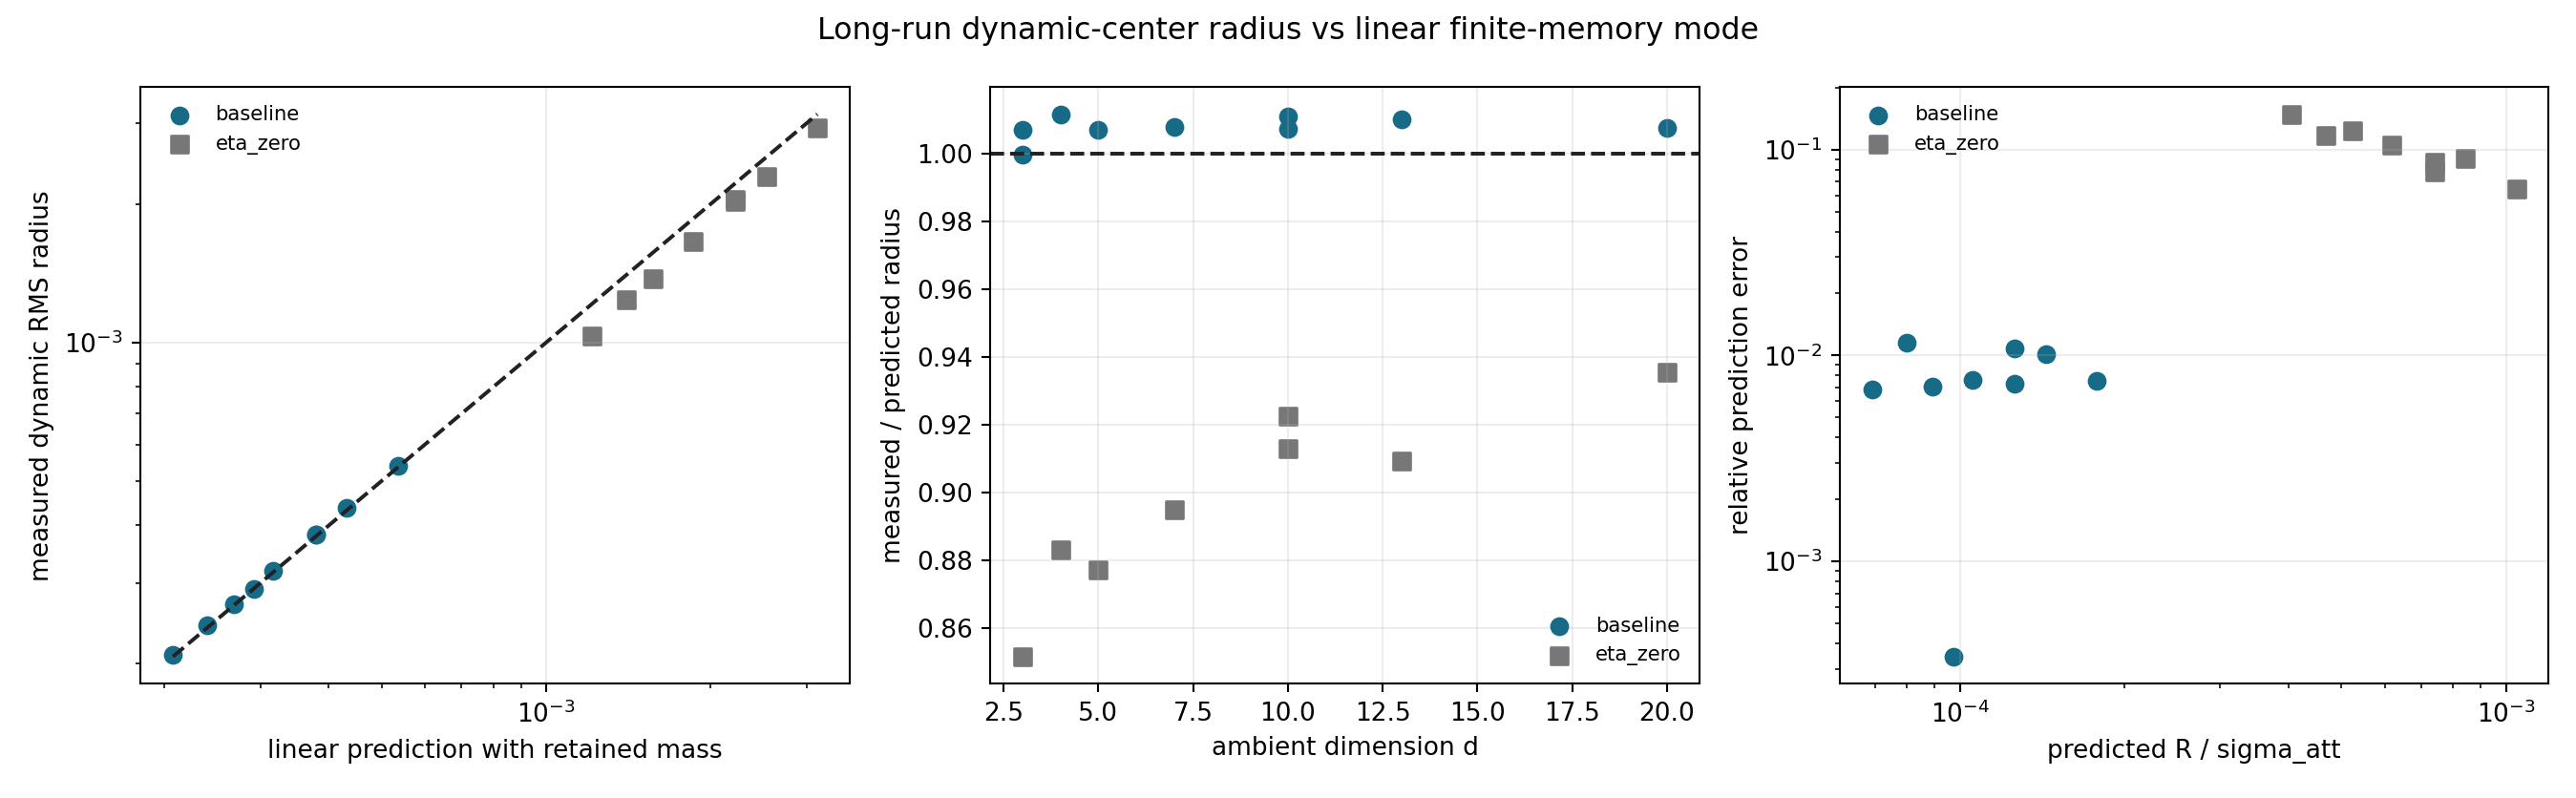
\includegraphics[width=\linewidth]{../../../figures/draft/scalar_hardening/linear_reconciliation_2026-07-19/linear_long_run_reconciliation.png}
  \caption{Measured co-moving radii compared with the finite-memory linear
  prediction. Active slices remain close to the diagonal across ambient
  dimension and run length. The $\eta=0$ controls are shown separately because
  the active-force formula is not an exact identity for their finite-window
  trace estimator.}
  \label{fig:linear_reconciliation}
\end{figure}

Two additional controls constrain the interpretation.
First, an attractive single-scale kernel and the earlier two-scale kernel
produce numerically indistinguishable scalar observables when matched by
their local restoring curvature.
The repulsive component is therefore not identified by the compact branch in
the sampled Taylor regime.
Second, increasing the predicted radius to $R_{\mathrm{lin}}/L=0.3$ produces a
seed-stable $6.2\%$ superlinear radius correction but no corresponding
memory-shape transition.
The preregistered composite decision remains inconclusive, while its
residence-based supports are either scale-dependent or saturated in the
$\eta=0$ control.

The covariance participation dimension of an isotropic cloud approaches the
supplied ambient dimension.
Consequently, a value near three in a three-dimensional embedding is an
expected shape check, not evidence for dimension selection, and is not used as
a primary result here.

\section{Criteria Beyond the Null Model}

We use \emph{localized memory cloud} for the descriptive state established
above.
The project term \emph{dynamical knot} is reserved for a stronger finding: a
nonlinear metastable regime that survives comparison with
Eq.~(\ref{eq:relative_mode}) and matched no-feedback controls.
For a region $\mathcal K\subset\Omega$, one possible observable is
\begin{equation}
M_n(\mathcal K)=\int_{\mathcal K}\rho_n(x)\,dx .
\end{equation}
However, elevated or long-lived $M_n(\mathcal K)$ is discriminating only when
the region definition scales with the cloud and the same statistic is not
saturated under the null.

A stronger test uses reduced features of the augmented state and estimates a
lagged transfer operator.
Almost-invariant sets or nontrivial slow modes can then be compared across
lag, discretization, seeds, and matched controls
\cite{FroylandLloydSantitissadeekorn2010,NoeNuske2013,
NoeWuPrinzPlattner2013}.
For an eigenvalue $\mu_i(\tau)$, the implied rate is
\begin{equation}
\Gamma_i(\tau)=-\frac{1}{\tau}\log|\mu_i(\tau)|.
\end{equation}
A local frozen-memory Hessian gives an OU approximation to such relaxation,
but it does not establish metastability by itself.
When a relaxation rate is independently identified, the dimensionless ratio
\begin{equation}
\widehat{\Gamma}=\frac{\sigma^2}{D}\Gamma_{\mathrm{rel}}
\end{equation}
compares relaxation with diffusion on the deposition scale.
No physical mass interpretation follows without an additional operational
calibration.

\section{Discussion}

The model provides a transparent field-valued Markov embedding of a
self-interacting trajectory with exponential forgetting.
Its main present numerical result is not a nonlinear knot claim.
It is the more discriminating finding that the scalar compact branch is a
co-moving relaxation cloud quantitatively controlled by the exact linear
center-relative mode over the tested long-run slices.

This negative separation is useful: future mechanisms must produce an
observable that the linear mode and matched controls cannot reproduce.
Candidate tests include a scale-aware almost-invariant set, a reproducible
nonlinear bifurcation, or a relational response channel with independently
evolved source and target states.
The current equations do not establish physical spacetime, finite signal
speed, dimension selection, quantum dynamics, particle structure, or
calibrated mass.

\begin{acknowledgments}
The author thanks colleagues for valuable feedback and discussion.
\end{acknowledgments}

\bibliographystyle{apsrev4-2}
\bibliography{references}

\end{document}
